% ===================================================================
%  并排的子图（(a) 总体比较/雷达图，(b) 大洲覆盖率）
% ===================================================================
\begin{figure}[t!]
    \centering % 将 figure 内的所有内容整体居中

    % ----- (a) 总体比较：雷达图 -----
    \begin{subfigure}[c]{0.48\linewidth}
        \centering
        
\includegraphics[width=1.0\linewidth]{radar_chart.pdf}
        \caption{Overall comparison.} % 子图 (a) 的小标题
        \label{fig:radar_metrics}           % 子图 (a) 的引用标签
    \end{subfigure}
    \hfill % 在左右两部分之间添加一个弹性的空白
    % ----- (b) 大洲覆盖率图表 -----
    \begin{subfigure}[c]{0.51\linewidth}
        \centering
        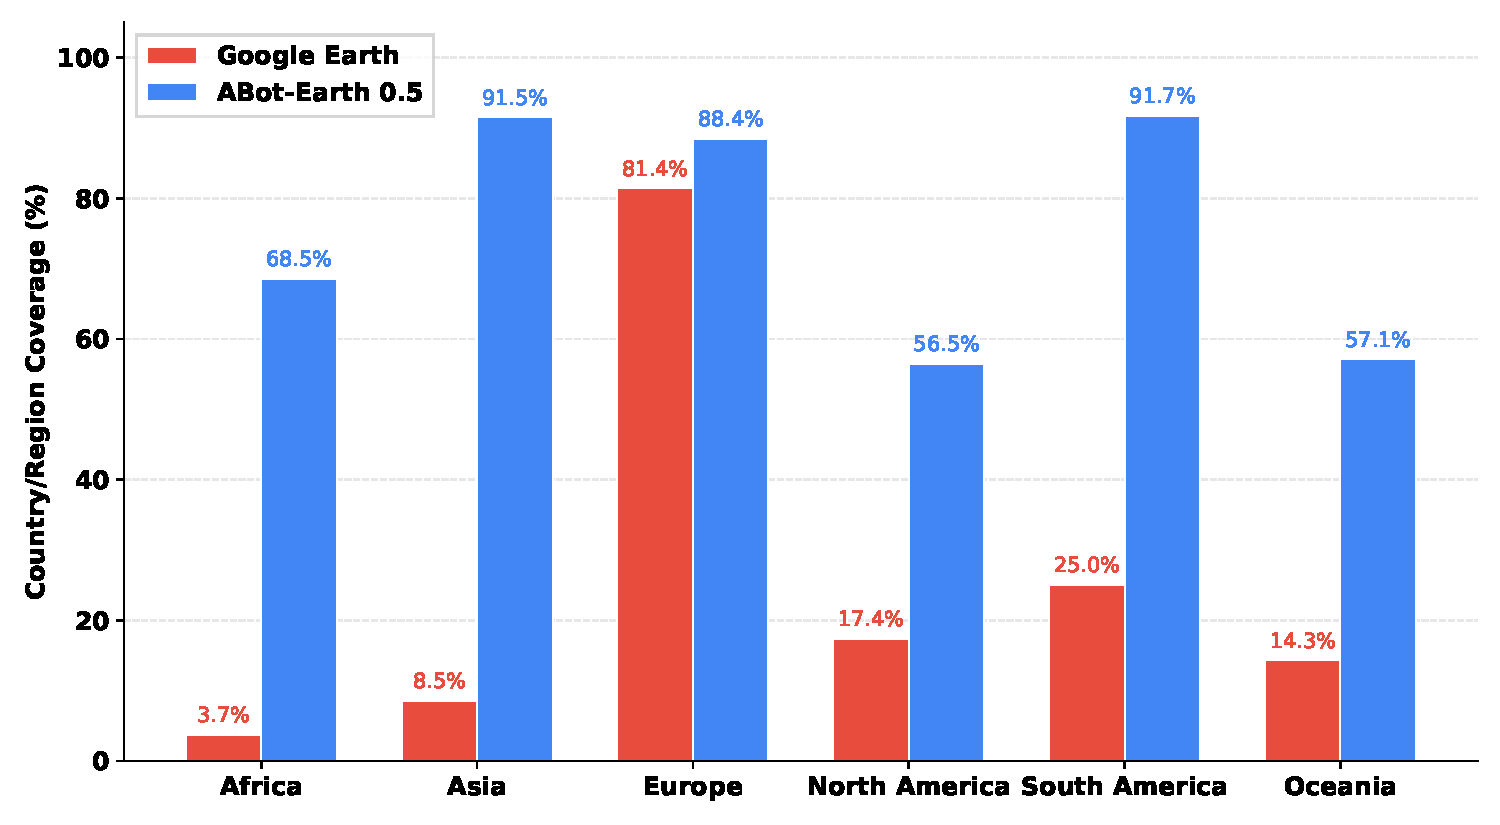
\includegraphics[width=1.0\linewidth]{continent_chart.pdf}
        \caption{Continental 3D coverage comparison.} % 子图 (b) 的小标题
        \label{fig:continent_coverage}      % 子图 (b) 的引用标签
    \end{subfigure}

    % 更新后的总标题
    \caption{Comparative analysis of \method{} and Google Earth. (a) Overall comparison of key system metrics and user-rated visual quality, including geometry, texture, and aesthetics. (b) Continental 3D coverage comparison, highlighting the broader reach of \method{} across all continents.}
    \label{fig:system_comparison} % 给整个 figure 一个总引用标签

\end{figure}
% ===================================================================
